\chapter{Approach}
\label{sec:approach}

All time synchronization algorithms have some inherent error, because
it is not possible to perfectly match time across a network. Some
algorithms are able to provide an uncertainty that upper-bounds that
error. The most common NTP implementation, ntpd, supports precisely
this. Specifically, it uses packet round trip time between clients and
the NTP server to provide an upper bound on error. It performs very
well with good clocks and network links, but degrades gracefully when
those are absent (see Chapter~\ref{sec:results} for a detailed
investigation of this point). This snapshot algorithm relies on having
a time synchronization algorithm capable of providing upper bounds.


\section{Phases}
There are four phases involved in this algorithm:

\begin{enumerate}

\item \emph{Synchronization}

  During the synchronization phase, all nodes run a supported time
  synchronization algorithm. All nodes attempts to synchronize their
  internal clocks with a single, common master
  clock\footnotemark. Administrative messages are also exchanged
  during this phase. These messages include scheduling future snapshot
  times. These messages could be inserted into already-extant messages
  such as heartbeat messages.

  \footnotetext{Multiple NTP servers may also be used, but they must
    all synchronize to the same root, or \textit{stratum 1}, NTP
    server. Otherwise, the NTP uncertainties will not necessarily
    provide overlapping freeze windows}

\item \emph{Freeze}
  
  When a node is frozen, it holds write confirmations. Incoming writes
  may be processed, but completion is not acknowledged until the end
  of the freeze.
  
  Let $U_i$ be the uncertainty in node $i$'s current time (i.e. the
  error bounds the time synchronization algorithm is able to
  determine), and $T$ be the scheduled snapshot time. Node $i$ begins
  its freeze when its clock reads $T - U_i$, and completes it when its
  clock reads $T + U_i$, guaranteeing that the master clock's $T$ is
  captured in the freeze window for all $i$ (Chapter~\ref{sec:proof}).

\item \emph{Confirmation}

  Before a snapshot may be marked as successful, the data center must
  wait a short period. This allows any sudden clock desynchronization
  events or node failures to be detected and consistency checked. The
  Ceph cluster must verify that, for every node failure during the
  snapshot, at least one other replica of that node's data did not
  fail. This is enough data to recover a snapshot
  (Chapter~\ref{sec:proof}).  If no uncrecoverable inconsistencies are
  found, the snapshot is marked as successful.

\item \emph{Replication}
  
  Finally, the data in the Ceph cluster as it existed at the time of
  the snapshot may begin being replicated to a remote Ceph cluster
  (provided the confirmation phase succeeded).  The first step in
  taking a snapshot is simply writing down a marker in a node's log
  separating pre- and post-snapshot writes. It is therefore
  straightforward either to do a full snapshot, or just capture the
  difference since the last good snapshot (the last snapshot
  log-marker).
  
  While replication is underway, the next synchronization phase begins.

\end{enumerate}

By using the uncertainty in a time synchronization algorithm in this
manner, we are able to have a per-node \textit{safety buffer} in each
freeze period, as shown in figure~\ref{fig:safety-buff}.

\begin{figure}
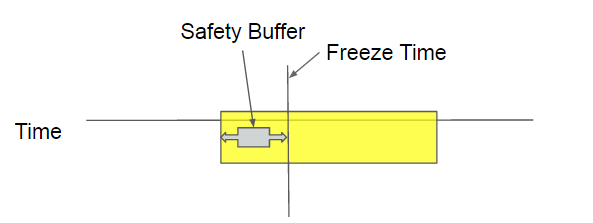
\includegraphics[width=0.8\textwidth]{safety-diagram.png}
\caption{~The gap between the edge of the freeze window and the point at which the NTP server believes the snapshot is scheduled is called the safety buffer}
\label{fig:safety-buff}
\end{figure}

\section{Overlapping freeze windows}

The freeze windows for our algorithm are designed to ensure
that there is some point in time at which all nodes in the cluster are
frozen. Each node knows the intended freeze time. However, since their
clocks are not perfect, they cannot know exactly when they have reached it.

Recall that our algorithm calls for each node to start its freeze
window when its clock reads $T - U_i$, and completes it when its clock
reads $T + U_i$, where $T$ is the freeze time and $U_i$ is the time
synchronization method's (e.g. NTP) uncertainty at that time.  Since
our chosen time synchronization method guarantees that the real time
$T$ will be within the uncertainty bounds of when the node's clock
reads $T$, we can be sure that each node will be frozen when the NTP
server's clock shows the scheduled snapshot time. Therefore, we can be
certain that their freeze windows overlap.
Figure~\ref{fig:overlapping-windows} demonstrates this concept with
four freeze windows overlapping at the freeze time of 8pm.

\begin{figure}[h]
  \centering
  \caption{}
  \label{fig:overlapping-windows}
  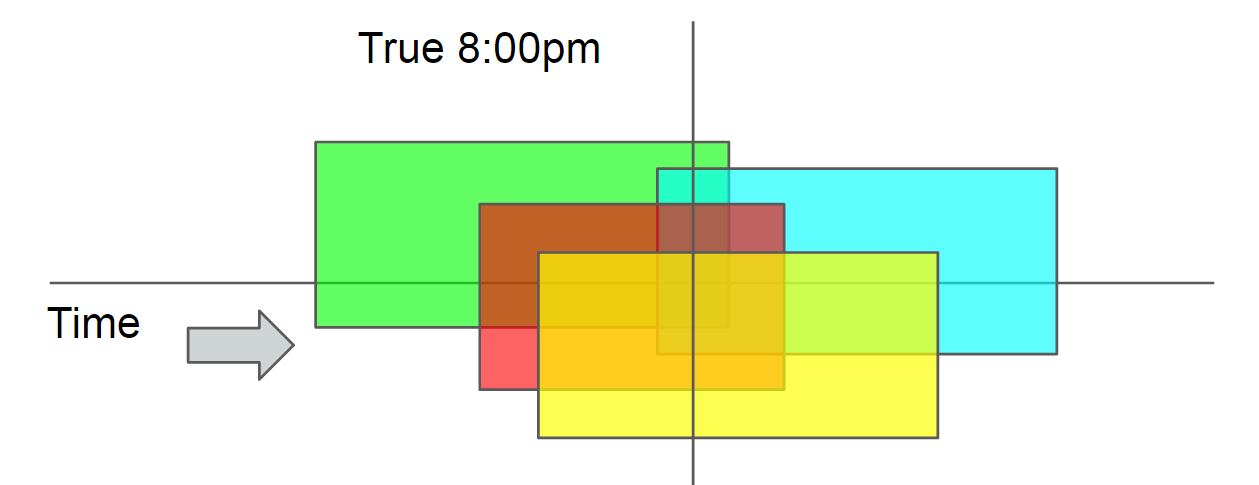
\includegraphics[width=0.8\textwidth]{overlapping-windows.png}
\end{figure}
